% v37 architecture — block-level overview (paper main figure).
% Compile standalone:  pdflatex architecture_v37.tex
% Or % v37 architecture — block-level overview (paper main figure).
% Compile standalone:  pdflatex architecture_v37.tex
% Or % v37 architecture — block-level overview (paper main figure).
% Compile standalone:  pdflatex architecture_v37.tex
% Or % v37 architecture — block-level overview (paper main figure).
% Compile standalone:  pdflatex architecture_v37.tex
% Or \input{figures/architecture_v37} inside the paper .tex (wrap in \begin{figure}).
\documentclass[tikz,border=8pt]{standalone}
\usepackage{tikz}
\usepackage{amsmath}
\usetikzlibrary{positioning,arrows.meta,calc,fit,backgrounds,shapes.geometric,decorations.pathreplacing}

\begin{document}
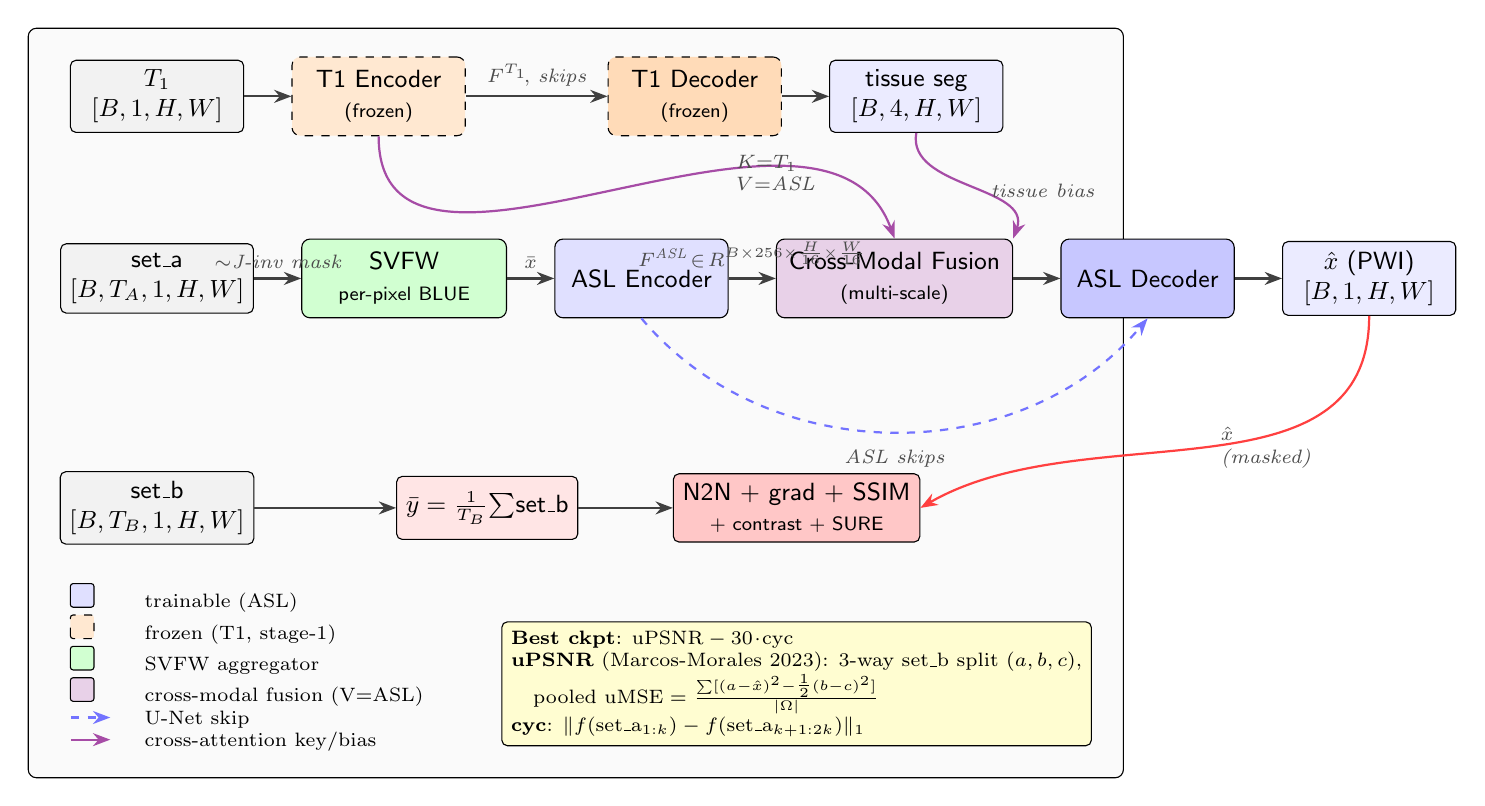
\begin{tikzpicture}[
    font=\small\sffamily,
    >={Stealth[length=2.2mm]},
    node distance=4mm and 6mm,
    % --- block styles -----------------------------------------------------
    input/.style   ={draw, rounded corners=2pt, fill=gray!10,
                     minimum width=22mm, minimum height=8mm, align=center},
    enc/.style     ={draw, rounded corners=3pt, fill=blue!12,
                     minimum width=22mm, minimum height=10mm, align=center},
    dec/.style     ={draw, rounded corners=3pt, fill=blue!22,
                     minimum width=22mm, minimum height=10mm, align=center},
    t1enc/.style   ={draw, rounded corners=3pt, fill=orange!18, dashed,
                     minimum width=22mm, minimum height=10mm, align=center},
    t1dec/.style   ={draw, rounded corners=3pt, fill=orange!28, dashed,
                     minimum width=22mm, minimum height=10mm, align=center},
    svfw/.style    ={draw, rounded corners=3pt, fill=green!18,
                     minimum width=26mm, minimum height=10mm, align=center},
    fusion/.style  ={draw, rounded corners=3pt, fill=violet!18,
                     minimum width=30mm, minimum height=10mm, align=center},
    target/.style  ={draw, rounded corners=2pt, fill=red!10,
                     minimum width=22mm, minimum height=8mm, align=center},
    loss/.style    ={draw, rounded corners=2pt, fill=red!22,
                     minimum width=24mm, minimum height=8mm, align=center},
    output/.style  ={draw, rounded corners=2pt, fill=blue!8,
                     minimum width=22mm, minimum height=8mm, align=center},
    note/.style    ={font=\scriptsize\itshape, gray!60!black},
    arr/.style     ={->, thick, black!75},
    skip/.style    ={->, thick, blue!55, dashed},
    cross/.style   ={->, thick, violet!70},
    grad/.style    ={->, thick, red!75},
]

% =============================================================
%   Row 1 — T1 branch (frozen, stage-1 pretrained)
% =============================================================
\node[input]   (t1in)   {$T_1$ \\ $[B,1,H,W]$};
\node[t1enc, right=of t1in]                 (t1enc)  {T1 Encoder \\ \scriptsize (frozen)};
\node[t1dec, right=18mm of t1enc]            (t1dec)  {T1 Decoder \\ \scriptsize (frozen)};
\node[output, right=of t1dec]                (t1seg)  {tissue seg \\ $[B,4,H,W]$};

\draw[arr] (t1in)  -- (t1enc);
\draw[arr] (t1enc) -- node[above,note]{$F^{T_1}\!,\,\text{skips}$} (t1dec);
\draw[arr] (t1dec) -- (t1seg);

% =============================================================
%   Row 2 — ASL branch (trainable)
% =============================================================
\node[input,  below=14mm of t1in]            (seta)   {set\_a \\ $[B,T_A,1,H,W]$};
\node[svfw,   right=of seta]                 (svfw)   {SVFW \\ \scriptsize per-pixel BLUE};
\node[enc,    right=of svfw]                 (aslenc) {ASL Encoder};
\node[fusion, right=of aslenc]               (fuse)   {Cross-Modal Fusion \\ \scriptsize (multi-scale)};
\node[dec,    right=of fuse]                 (asldec) {ASL Decoder};
\node[output, right=of asldec]               (recon)  {$\hat{x}$ (PWI) \\ $[B,1,H,W]$};

\draw[arr] (seta)   -- node[above,note]{$\sim$J-inv mask} (svfw);
\draw[arr] (svfw)   -- node[above,note]{$\bar{x}$} (aslenc);
\draw[arr] (aslenc) -- node[above,note]{$F^{\text{ASL}}\!\in\!\mathbb{R}^{B\times256\times\frac{H}{16}\times\frac{W}{16}}$} (fuse);
\draw[arr] (fuse)   -- (asldec);
\draw[arr] (asldec) -- (recon);

% U-Net skips ASL-only (decoder reuses ASL encoder skips, NOT T1 skips)
\draw[skip] (aslenc.south) to[out=-50,in=-130] node[below=1mm,note]{ASL skips} (asldec.south);

% Cross-modal: T1 features feed K, tissue seg provides similarity bias; V = ASL (anti-hallucination)
\draw[cross] (t1enc.south) to[out=-90,in=110] node[pos=0.65,right=1mm,note,align=left]{$K{=}T_1$\\$V{=}\text{ASL}$} (fuse.north);
\draw[cross] (t1seg.south) to[out=-100,in=70] node[pos=0.55,right=0.5mm,note]{tissue bias} (fuse.north east);

% =============================================================
%   Row 3 — N2N target + losses
% =============================================================
\node[input,  below=20mm of seta]            (setb)   {set\_b \\ $[B,T_B,1,H,W]$};
\node[target, right=18mm of setb]            (mean)   {$\bar{y}=\tfrac{1}{T_B}\!\sum\!\text{set\_b}$};
\node[loss,   right=12mm of mean]            (lossn)  {N2N + grad + SSIM \\ \scriptsize + contrast + SURE};

\draw[arr] (setb) -- (mean);
\draw[arr] (mean) -- (lossn);
\draw[grad] (recon.south) to[out=-90,in=30] node[right=0.5mm,note,align=left]{$\hat{x}$\\(masked)} (lossn.east);

% =============================================================
%   Validation criterion box
% =============================================================
\node[draw, rounded corners=2pt, fill=yellow!18,
      below=10mm of lossn, minimum width=68mm, align=left, font=\scriptsize]
      (val) {%
      \textbf{Best ckpt}: $\text{uPSNR}-30\!\cdot\!\text{cyc}$ \\
      \textbf{uPSNR} (Marcos-Morales 2023): 3-way set\_b split $(a,b,c)$, \\
      \quad pooled $\text{uMSE}=\frac{\sum[(a-\hat{x})^2-\tfrac12(b-c)^2]}{|\Omega|}$ \\
      \textbf{cyc}: $\|f(\text{set\_a}_{1:k})-f(\text{set\_a}_{k+1:2k})\|_1$};

% =============================================================
%   Legend
% =============================================================
\begin{scope}[on background layer]
  \node[draw, rounded corners=3pt, fill=gray!4,
        fit=(t1in)(t1seg)(setb)(val)(lossn),
        inner sep=4mm] (bg) {};
\end{scope}

\node[font=\scriptsize, anchor=south west] at ([xshift=2mm,yshift=2mm]bg.south west) {%
  \begin{tabular}{ll}
    \tikz\draw[fill=blue!12,rounded corners=1pt](0,0) rectangle (3mm,3mm); & trainable (ASL) \\
    \tikz\draw[fill=orange!18,dashed,rounded corners=1pt](0,0) rectangle (3mm,3mm); & frozen (T1, stage-1) \\
    \tikz\draw[fill=green!18,rounded corners=1pt](0,0) rectangle (3mm,3mm); & SVFW aggregator \\
    \tikz\draw[fill=violet!18,rounded corners=1pt](0,0) rectangle (3mm,3mm); & cross-modal fusion (V=ASL) \\
    \tikz\draw[->,thick,blue!55,dashed] (0,1.5mm) -- (5mm,1.5mm); & U-Net skip \\
    \tikz\draw[->,thick,violet!70] (0,1.5mm) -- (5mm,1.5mm); & cross-attention key/bias \\
  \end{tabular}};

\end{tikzpicture}
\end{document}
 inside the paper .tex (wrap in \begin{figure}).
\documentclass[tikz,border=8pt]{standalone}
\usepackage{tikz}
\usepackage{amsmath}
\usetikzlibrary{positioning,arrows.meta,calc,fit,backgrounds,shapes.geometric,decorations.pathreplacing}

\begin{document}
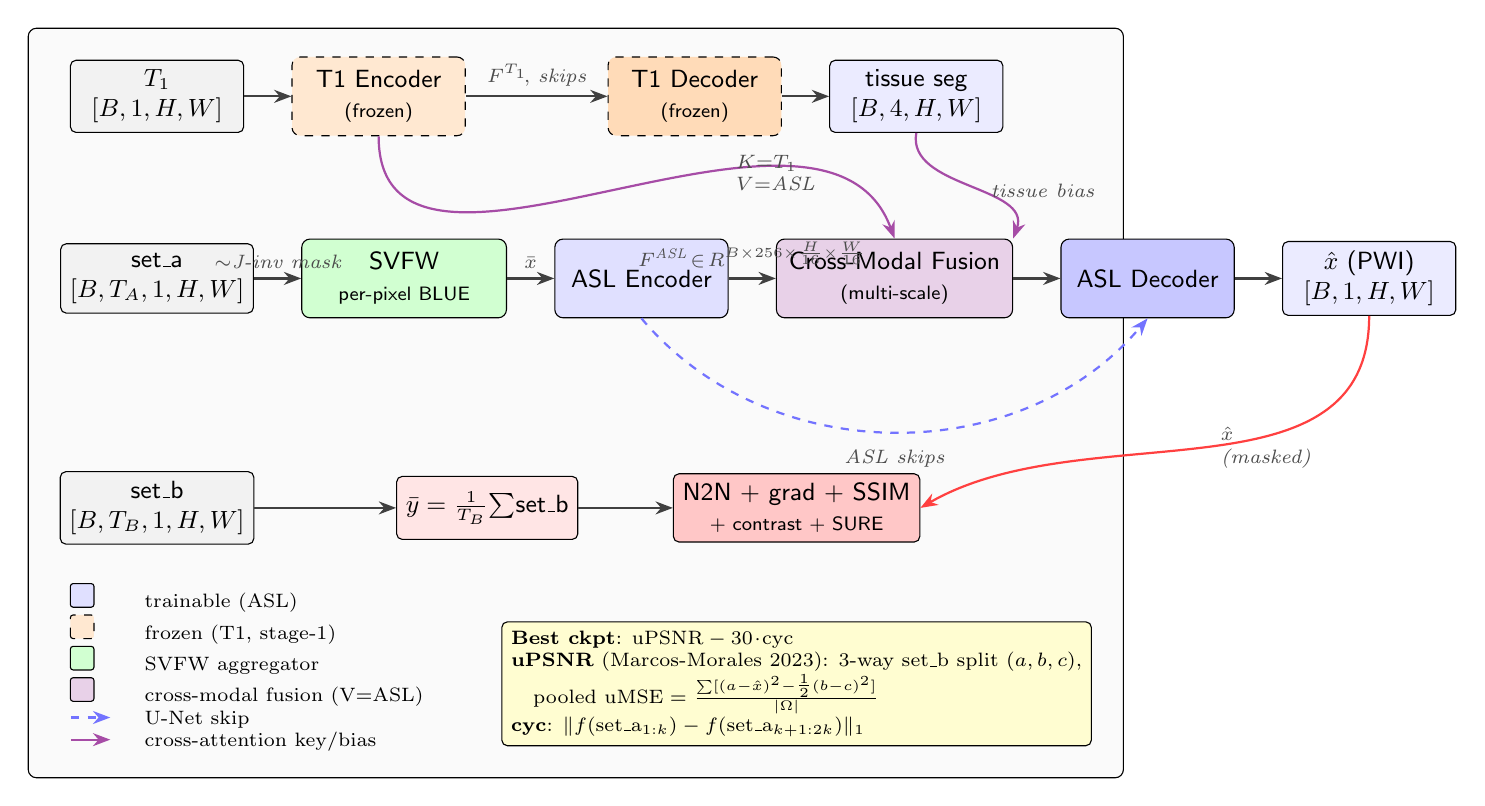
\begin{tikzpicture}[
    font=\small\sffamily,
    >={Stealth[length=2.2mm]},
    node distance=4mm and 6mm,
    % --- block styles -----------------------------------------------------
    input/.style   ={draw, rounded corners=2pt, fill=gray!10,
                     minimum width=22mm, minimum height=8mm, align=center},
    enc/.style     ={draw, rounded corners=3pt, fill=blue!12,
                     minimum width=22mm, minimum height=10mm, align=center},
    dec/.style     ={draw, rounded corners=3pt, fill=blue!22,
                     minimum width=22mm, minimum height=10mm, align=center},
    t1enc/.style   ={draw, rounded corners=3pt, fill=orange!18, dashed,
                     minimum width=22mm, minimum height=10mm, align=center},
    t1dec/.style   ={draw, rounded corners=3pt, fill=orange!28, dashed,
                     minimum width=22mm, minimum height=10mm, align=center},
    svfw/.style    ={draw, rounded corners=3pt, fill=green!18,
                     minimum width=26mm, minimum height=10mm, align=center},
    fusion/.style  ={draw, rounded corners=3pt, fill=violet!18,
                     minimum width=30mm, minimum height=10mm, align=center},
    target/.style  ={draw, rounded corners=2pt, fill=red!10,
                     minimum width=22mm, minimum height=8mm, align=center},
    loss/.style    ={draw, rounded corners=2pt, fill=red!22,
                     minimum width=24mm, minimum height=8mm, align=center},
    output/.style  ={draw, rounded corners=2pt, fill=blue!8,
                     minimum width=22mm, minimum height=8mm, align=center},
    note/.style    ={font=\scriptsize\itshape, gray!60!black},
    arr/.style     ={->, thick, black!75},
    skip/.style    ={->, thick, blue!55, dashed},
    cross/.style   ={->, thick, violet!70},
    grad/.style    ={->, thick, red!75},
]

% =============================================================
%   Row 1 — T1 branch (frozen, stage-1 pretrained)
% =============================================================
\node[input]   (t1in)   {$T_1$ \\ $[B,1,H,W]$};
\node[t1enc, right=of t1in]                 (t1enc)  {T1 Encoder \\ \scriptsize (frozen)};
\node[t1dec, right=18mm of t1enc]            (t1dec)  {T1 Decoder \\ \scriptsize (frozen)};
\node[output, right=of t1dec]                (t1seg)  {tissue seg \\ $[B,4,H,W]$};

\draw[arr] (t1in)  -- (t1enc);
\draw[arr] (t1enc) -- node[above,note]{$F^{T_1}\!,\,\text{skips}$} (t1dec);
\draw[arr] (t1dec) -- (t1seg);

% =============================================================
%   Row 2 — ASL branch (trainable)
% =============================================================
\node[input,  below=14mm of t1in]            (seta)   {set\_a \\ $[B,T_A,1,H,W]$};
\node[svfw,   right=of seta]                 (svfw)   {SVFW \\ \scriptsize per-pixel BLUE};
\node[enc,    right=of svfw]                 (aslenc) {ASL Encoder};
\node[fusion, right=of aslenc]               (fuse)   {Cross-Modal Fusion \\ \scriptsize (multi-scale)};
\node[dec,    right=of fuse]                 (asldec) {ASL Decoder};
\node[output, right=of asldec]               (recon)  {$\hat{x}$ (PWI) \\ $[B,1,H,W]$};

\draw[arr] (seta)   -- node[above,note]{$\sim$J-inv mask} (svfw);
\draw[arr] (svfw)   -- node[above,note]{$\bar{x}$} (aslenc);
\draw[arr] (aslenc) -- node[above,note]{$F^{\text{ASL}}\!\in\!\mathbb{R}^{B\times256\times\frac{H}{16}\times\frac{W}{16}}$} (fuse);
\draw[arr] (fuse)   -- (asldec);
\draw[arr] (asldec) -- (recon);

% U-Net skips ASL-only (decoder reuses ASL encoder skips, NOT T1 skips)
\draw[skip] (aslenc.south) to[out=-50,in=-130] node[below=1mm,note]{ASL skips} (asldec.south);

% Cross-modal: T1 features feed K, tissue seg provides similarity bias; V = ASL (anti-hallucination)
\draw[cross] (t1enc.south) to[out=-90,in=110] node[pos=0.65,right=1mm,note,align=left]{$K{=}T_1$\\$V{=}\text{ASL}$} (fuse.north);
\draw[cross] (t1seg.south) to[out=-100,in=70] node[pos=0.55,right=0.5mm,note]{tissue bias} (fuse.north east);

% =============================================================
%   Row 3 — N2N target + losses
% =============================================================
\node[input,  below=20mm of seta]            (setb)   {set\_b \\ $[B,T_B,1,H,W]$};
\node[target, right=18mm of setb]            (mean)   {$\bar{y}=\tfrac{1}{T_B}\!\sum\!\text{set\_b}$};
\node[loss,   right=12mm of mean]            (lossn)  {N2N + grad + SSIM \\ \scriptsize + contrast + SURE};

\draw[arr] (setb) -- (mean);
\draw[arr] (mean) -- (lossn);
\draw[grad] (recon.south) to[out=-90,in=30] node[right=0.5mm,note,align=left]{$\hat{x}$\\(masked)} (lossn.east);

% =============================================================
%   Validation criterion box
% =============================================================
\node[draw, rounded corners=2pt, fill=yellow!18,
      below=10mm of lossn, minimum width=68mm, align=left, font=\scriptsize]
      (val) {%
      \textbf{Best ckpt}: $\text{uPSNR}-30\!\cdot\!\text{cyc}$ \\
      \textbf{uPSNR} (Marcos-Morales 2023): 3-way set\_b split $(a,b,c)$, \\
      \quad pooled $\text{uMSE}=\frac{\sum[(a-\hat{x})^2-\tfrac12(b-c)^2]}{|\Omega|}$ \\
      \textbf{cyc}: $\|f(\text{set\_a}_{1:k})-f(\text{set\_a}_{k+1:2k})\|_1$};

% =============================================================
%   Legend
% =============================================================
\begin{scope}[on background layer]
  \node[draw, rounded corners=3pt, fill=gray!4,
        fit=(t1in)(t1seg)(setb)(val)(lossn),
        inner sep=4mm] (bg) {};
\end{scope}

\node[font=\scriptsize, anchor=south west] at ([xshift=2mm,yshift=2mm]bg.south west) {%
  \begin{tabular}{ll}
    \tikz\draw[fill=blue!12,rounded corners=1pt](0,0) rectangle (3mm,3mm); & trainable (ASL) \\
    \tikz\draw[fill=orange!18,dashed,rounded corners=1pt](0,0) rectangle (3mm,3mm); & frozen (T1, stage-1) \\
    \tikz\draw[fill=green!18,rounded corners=1pt](0,0) rectangle (3mm,3mm); & SVFW aggregator \\
    \tikz\draw[fill=violet!18,rounded corners=1pt](0,0) rectangle (3mm,3mm); & cross-modal fusion (V=ASL) \\
    \tikz\draw[->,thick,blue!55,dashed] (0,1.5mm) -- (5mm,1.5mm); & U-Net skip \\
    \tikz\draw[->,thick,violet!70] (0,1.5mm) -- (5mm,1.5mm); & cross-attention key/bias \\
  \end{tabular}};

\end{tikzpicture}
\end{document}
 inside the paper .tex (wrap in \begin{figure}).
\documentclass[tikz,border=8pt]{standalone}
\usepackage{tikz}
\usepackage{amsmath}
\usetikzlibrary{positioning,arrows.meta,calc,fit,backgrounds,shapes.geometric,decorations.pathreplacing}

\begin{document}
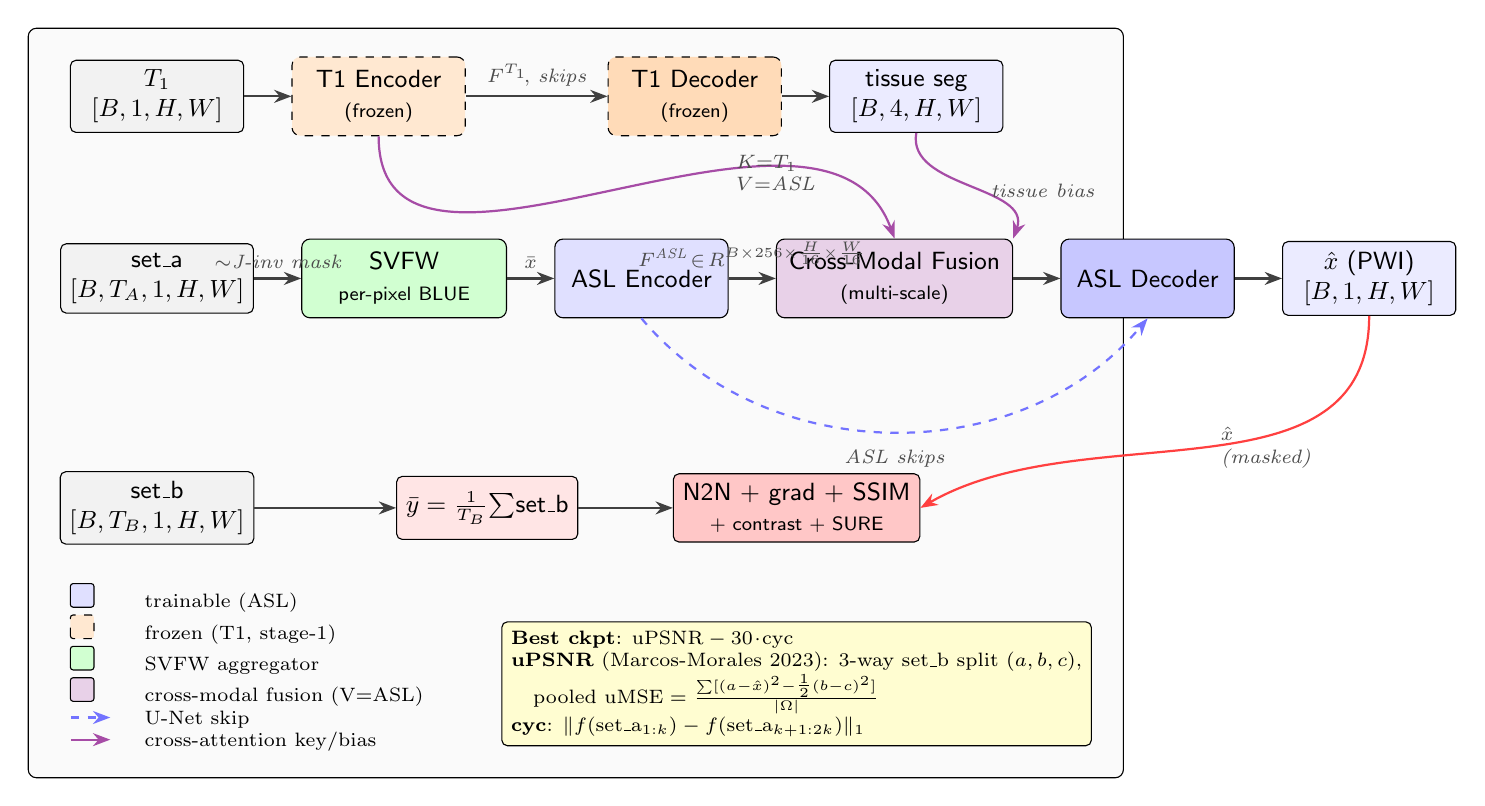
\begin{tikzpicture}[
    font=\small\sffamily,
    >={Stealth[length=2.2mm]},
    node distance=4mm and 6mm,
    % --- block styles -----------------------------------------------------
    input/.style   ={draw, rounded corners=2pt, fill=gray!10,
                     minimum width=22mm, minimum height=8mm, align=center},
    enc/.style     ={draw, rounded corners=3pt, fill=blue!12,
                     minimum width=22mm, minimum height=10mm, align=center},
    dec/.style     ={draw, rounded corners=3pt, fill=blue!22,
                     minimum width=22mm, minimum height=10mm, align=center},
    t1enc/.style   ={draw, rounded corners=3pt, fill=orange!18, dashed,
                     minimum width=22mm, minimum height=10mm, align=center},
    t1dec/.style   ={draw, rounded corners=3pt, fill=orange!28, dashed,
                     minimum width=22mm, minimum height=10mm, align=center},
    svfw/.style    ={draw, rounded corners=3pt, fill=green!18,
                     minimum width=26mm, minimum height=10mm, align=center},
    fusion/.style  ={draw, rounded corners=3pt, fill=violet!18,
                     minimum width=30mm, minimum height=10mm, align=center},
    target/.style  ={draw, rounded corners=2pt, fill=red!10,
                     minimum width=22mm, minimum height=8mm, align=center},
    loss/.style    ={draw, rounded corners=2pt, fill=red!22,
                     minimum width=24mm, minimum height=8mm, align=center},
    output/.style  ={draw, rounded corners=2pt, fill=blue!8,
                     minimum width=22mm, minimum height=8mm, align=center},
    note/.style    ={font=\scriptsize\itshape, gray!60!black},
    arr/.style     ={->, thick, black!75},
    skip/.style    ={->, thick, blue!55, dashed},
    cross/.style   ={->, thick, violet!70},
    grad/.style    ={->, thick, red!75},
]

% =============================================================
%   Row 1 — T1 branch (frozen, stage-1 pretrained)
% =============================================================
\node[input]   (t1in)   {$T_1$ \\ $[B,1,H,W]$};
\node[t1enc, right=of t1in]                 (t1enc)  {T1 Encoder \\ \scriptsize (frozen)};
\node[t1dec, right=18mm of t1enc]            (t1dec)  {T1 Decoder \\ \scriptsize (frozen)};
\node[output, right=of t1dec]                (t1seg)  {tissue seg \\ $[B,4,H,W]$};

\draw[arr] (t1in)  -- (t1enc);
\draw[arr] (t1enc) -- node[above,note]{$F^{T_1}\!,\,\text{skips}$} (t1dec);
\draw[arr] (t1dec) -- (t1seg);

% =============================================================
%   Row 2 — ASL branch (trainable)
% =============================================================
\node[input,  below=14mm of t1in]            (seta)   {set\_a \\ $[B,T_A,1,H,W]$};
\node[svfw,   right=of seta]                 (svfw)   {SVFW \\ \scriptsize per-pixel BLUE};
\node[enc,    right=of svfw]                 (aslenc) {ASL Encoder};
\node[fusion, right=of aslenc]               (fuse)   {Cross-Modal Fusion \\ \scriptsize (multi-scale)};
\node[dec,    right=of fuse]                 (asldec) {ASL Decoder};
\node[output, right=of asldec]               (recon)  {$\hat{x}$ (PWI) \\ $[B,1,H,W]$};

\draw[arr] (seta)   -- node[above,note]{$\sim$J-inv mask} (svfw);
\draw[arr] (svfw)   -- node[above,note]{$\bar{x}$} (aslenc);
\draw[arr] (aslenc) -- node[above,note]{$F^{\text{ASL}}\!\in\!\mathbb{R}^{B\times256\times\frac{H}{16}\times\frac{W}{16}}$} (fuse);
\draw[arr] (fuse)   -- (asldec);
\draw[arr] (asldec) -- (recon);

% U-Net skips ASL-only (decoder reuses ASL encoder skips, NOT T1 skips)
\draw[skip] (aslenc.south) to[out=-50,in=-130] node[below=1mm,note]{ASL skips} (asldec.south);

% Cross-modal: T1 features feed K, tissue seg provides similarity bias; V = ASL (anti-hallucination)
\draw[cross] (t1enc.south) to[out=-90,in=110] node[pos=0.65,right=1mm,note,align=left]{$K{=}T_1$\\$V{=}\text{ASL}$} (fuse.north);
\draw[cross] (t1seg.south) to[out=-100,in=70] node[pos=0.55,right=0.5mm,note]{tissue bias} (fuse.north east);

% =============================================================
%   Row 3 — N2N target + losses
% =============================================================
\node[input,  below=20mm of seta]            (setb)   {set\_b \\ $[B,T_B,1,H,W]$};
\node[target, right=18mm of setb]            (mean)   {$\bar{y}=\tfrac{1}{T_B}\!\sum\!\text{set\_b}$};
\node[loss,   right=12mm of mean]            (lossn)  {N2N + grad + SSIM \\ \scriptsize + contrast + SURE};

\draw[arr] (setb) -- (mean);
\draw[arr] (mean) -- (lossn);
\draw[grad] (recon.south) to[out=-90,in=30] node[right=0.5mm,note,align=left]{$\hat{x}$\\(masked)} (lossn.east);

% =============================================================
%   Validation criterion box
% =============================================================
\node[draw, rounded corners=2pt, fill=yellow!18,
      below=10mm of lossn, minimum width=68mm, align=left, font=\scriptsize]
      (val) {%
      \textbf{Best ckpt}: $\text{uPSNR}-30\!\cdot\!\text{cyc}$ \\
      \textbf{uPSNR} (Marcos-Morales 2023): 3-way set\_b split $(a,b,c)$, \\
      \quad pooled $\text{uMSE}=\frac{\sum[(a-\hat{x})^2-\tfrac12(b-c)^2]}{|\Omega|}$ \\
      \textbf{cyc}: $\|f(\text{set\_a}_{1:k})-f(\text{set\_a}_{k+1:2k})\|_1$};

% =============================================================
%   Legend
% =============================================================
\begin{scope}[on background layer]
  \node[draw, rounded corners=3pt, fill=gray!4,
        fit=(t1in)(t1seg)(setb)(val)(lossn),
        inner sep=4mm] (bg) {};
\end{scope}

\node[font=\scriptsize, anchor=south west] at ([xshift=2mm,yshift=2mm]bg.south west) {%
  \begin{tabular}{ll}
    \tikz\draw[fill=blue!12,rounded corners=1pt](0,0) rectangle (3mm,3mm); & trainable (ASL) \\
    \tikz\draw[fill=orange!18,dashed,rounded corners=1pt](0,0) rectangle (3mm,3mm); & frozen (T1, stage-1) \\
    \tikz\draw[fill=green!18,rounded corners=1pt](0,0) rectangle (3mm,3mm); & SVFW aggregator \\
    \tikz\draw[fill=violet!18,rounded corners=1pt](0,0) rectangle (3mm,3mm); & cross-modal fusion (V=ASL) \\
    \tikz\draw[->,thick,blue!55,dashed] (0,1.5mm) -- (5mm,1.5mm); & U-Net skip \\
    \tikz\draw[->,thick,violet!70] (0,1.5mm) -- (5mm,1.5mm); & cross-attention key/bias \\
  \end{tabular}};

\end{tikzpicture}
\end{document}
 inside the paper .tex (wrap in \begin{figure}).
\documentclass[tikz,border=8pt]{standalone}
\usepackage{tikz}
\usepackage{amsmath}
\usetikzlibrary{positioning,arrows.meta,calc,fit,backgrounds,shapes.geometric,decorations.pathreplacing}

\begin{document}
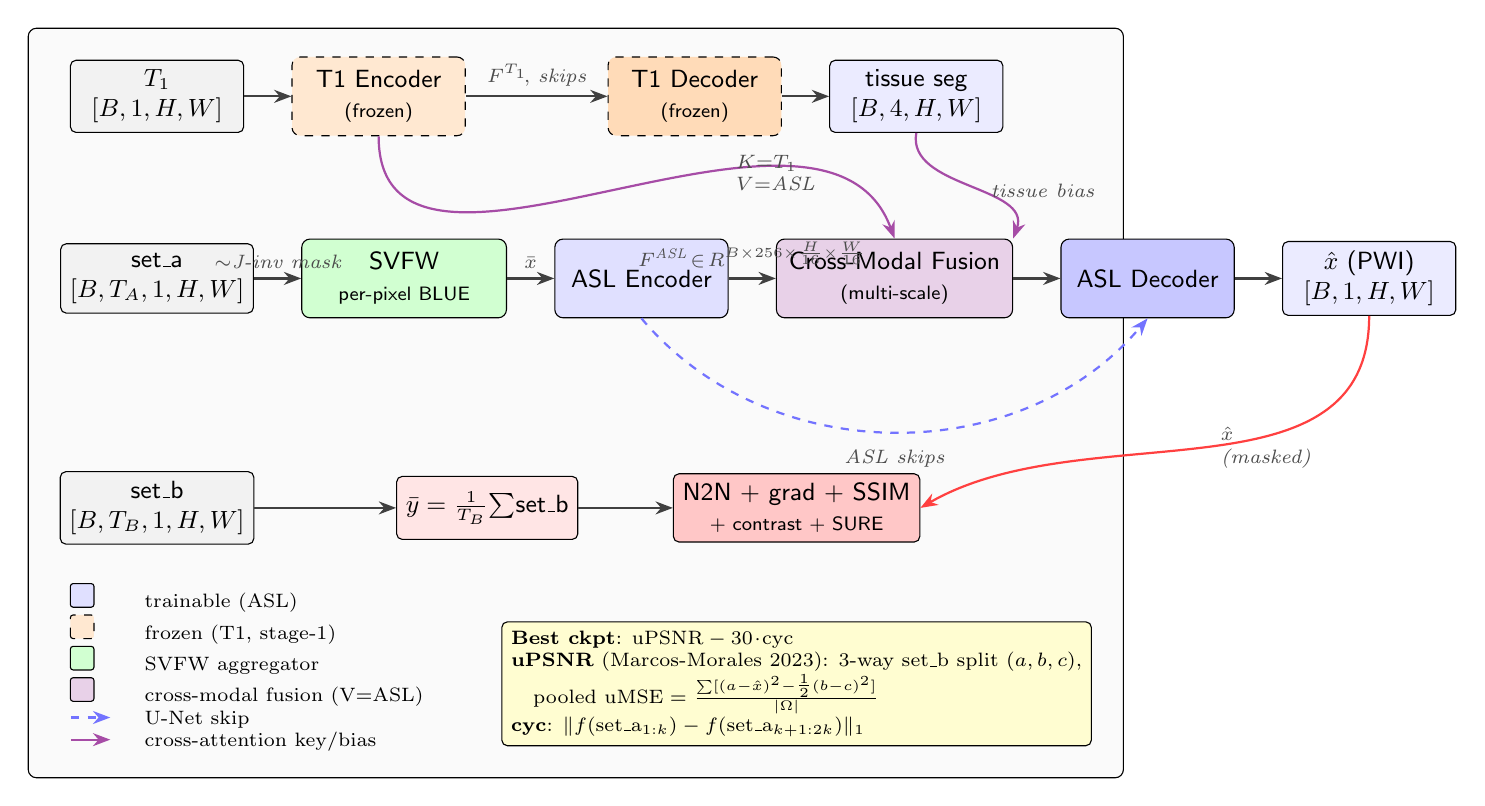
\begin{tikzpicture}[
    font=\small\sffamily,
    >={Stealth[length=2.2mm]},
    node distance=4mm and 6mm,
    % --- block styles -----------------------------------------------------
    input/.style   ={draw, rounded corners=2pt, fill=gray!10,
                     minimum width=22mm, minimum height=8mm, align=center},
    enc/.style     ={draw, rounded corners=3pt, fill=blue!12,
                     minimum width=22mm, minimum height=10mm, align=center},
    dec/.style     ={draw, rounded corners=3pt, fill=blue!22,
                     minimum width=22mm, minimum height=10mm, align=center},
    t1enc/.style   ={draw, rounded corners=3pt, fill=orange!18, dashed,
                     minimum width=22mm, minimum height=10mm, align=center},
    t1dec/.style   ={draw, rounded corners=3pt, fill=orange!28, dashed,
                     minimum width=22mm, minimum height=10mm, align=center},
    svfw/.style    ={draw, rounded corners=3pt, fill=green!18,
                     minimum width=26mm, minimum height=10mm, align=center},
    fusion/.style  ={draw, rounded corners=3pt, fill=violet!18,
                     minimum width=30mm, minimum height=10mm, align=center},
    target/.style  ={draw, rounded corners=2pt, fill=red!10,
                     minimum width=22mm, minimum height=8mm, align=center},
    loss/.style    ={draw, rounded corners=2pt, fill=red!22,
                     minimum width=24mm, minimum height=8mm, align=center},
    output/.style  ={draw, rounded corners=2pt, fill=blue!8,
                     minimum width=22mm, minimum height=8mm, align=center},
    note/.style    ={font=\scriptsize\itshape, gray!60!black},
    arr/.style     ={->, thick, black!75},
    skip/.style    ={->, thick, blue!55, dashed},
    cross/.style   ={->, thick, violet!70},
    grad/.style    ={->, thick, red!75},
]

% =============================================================
%   Row 1 — T1 branch (frozen, stage-1 pretrained)
% =============================================================
\node[input]   (t1in)   {$T_1$ \\ $[B,1,H,W]$};
\node[t1enc, right=of t1in]                 (t1enc)  {T1 Encoder \\ \scriptsize (frozen)};
\node[t1dec, right=18mm of t1enc]            (t1dec)  {T1 Decoder \\ \scriptsize (frozen)};
\node[output, right=of t1dec]                (t1seg)  {tissue seg \\ $[B,4,H,W]$};

\draw[arr] (t1in)  -- (t1enc);
\draw[arr] (t1enc) -- node[above,note]{$F^{T_1}\!,\,\text{skips}$} (t1dec);
\draw[arr] (t1dec) -- (t1seg);

% =============================================================
%   Row 2 — ASL branch (trainable)
% =============================================================
\node[input,  below=14mm of t1in]            (seta)   {set\_a \\ $[B,T_A,1,H,W]$};
\node[svfw,   right=of seta]                 (svfw)   {SVFW \\ \scriptsize per-pixel BLUE};
\node[enc,    right=of svfw]                 (aslenc) {ASL Encoder};
\node[fusion, right=of aslenc]               (fuse)   {Cross-Modal Fusion \\ \scriptsize (multi-scale)};
\node[dec,    right=of fuse]                 (asldec) {ASL Decoder};
\node[output, right=of asldec]               (recon)  {$\hat{x}$ (PWI) \\ $[B,1,H,W]$};

\draw[arr] (seta)   -- node[above,note]{$\sim$J-inv mask} (svfw);
\draw[arr] (svfw)   -- node[above,note]{$\bar{x}$} (aslenc);
\draw[arr] (aslenc) -- node[above,note]{$F^{\text{ASL}}\!\in\!\mathbb{R}^{B\times256\times\frac{H}{16}\times\frac{W}{16}}$} (fuse);
\draw[arr] (fuse)   -- (asldec);
\draw[arr] (asldec) -- (recon);

% U-Net skips ASL-only (decoder reuses ASL encoder skips, NOT T1 skips)
\draw[skip] (aslenc.south) to[out=-50,in=-130] node[below=1mm,note]{ASL skips} (asldec.south);

% Cross-modal: T1 features feed K, tissue seg provides similarity bias; V = ASL (anti-hallucination)
\draw[cross] (t1enc.south) to[out=-90,in=110] node[pos=0.65,right=1mm,note,align=left]{$K{=}T_1$\\$V{=}\text{ASL}$} (fuse.north);
\draw[cross] (t1seg.south) to[out=-100,in=70] node[pos=0.55,right=0.5mm,note]{tissue bias} (fuse.north east);

% =============================================================
%   Row 3 — N2N target + losses
% =============================================================
\node[input,  below=20mm of seta]            (setb)   {set\_b \\ $[B,T_B,1,H,W]$};
\node[target, right=18mm of setb]            (mean)   {$\bar{y}=\tfrac{1}{T_B}\!\sum\!\text{set\_b}$};
\node[loss,   right=12mm of mean]            (lossn)  {N2N + grad + SSIM \\ \scriptsize + contrast + SURE};

\draw[arr] (setb) -- (mean);
\draw[arr] (mean) -- (lossn);
\draw[grad] (recon.south) to[out=-90,in=30] node[right=0.5mm,note,align=left]{$\hat{x}$\\(masked)} (lossn.east);

% =============================================================
%   Validation criterion box
% =============================================================
\node[draw, rounded corners=2pt, fill=yellow!18,
      below=10mm of lossn, minimum width=68mm, align=left, font=\scriptsize]
      (val) {%
      \textbf{Best ckpt}: $\text{uPSNR}-30\!\cdot\!\text{cyc}$ \\
      \textbf{uPSNR} (Marcos-Morales 2023): 3-way set\_b split $(a,b,c)$, \\
      \quad pooled $\text{uMSE}=\frac{\sum[(a-\hat{x})^2-\tfrac12(b-c)^2]}{|\Omega|}$ \\
      \textbf{cyc}: $\|f(\text{set\_a}_{1:k})-f(\text{set\_a}_{k+1:2k})\|_1$};

% =============================================================
%   Legend
% =============================================================
\begin{scope}[on background layer]
  \node[draw, rounded corners=3pt, fill=gray!4,
        fit=(t1in)(t1seg)(setb)(val)(lossn),
        inner sep=4mm] (bg) {};
\end{scope}

\node[font=\scriptsize, anchor=south west] at ([xshift=2mm,yshift=2mm]bg.south west) {%
  \begin{tabular}{ll}
    \tikz\draw[fill=blue!12,rounded corners=1pt](0,0) rectangle (3mm,3mm); & trainable (ASL) \\
    \tikz\draw[fill=orange!18,dashed,rounded corners=1pt](0,0) rectangle (3mm,3mm); & frozen (T1, stage-1) \\
    \tikz\draw[fill=green!18,rounded corners=1pt](0,0) rectangle (3mm,3mm); & SVFW aggregator \\
    \tikz\draw[fill=violet!18,rounded corners=1pt](0,0) rectangle (3mm,3mm); & cross-modal fusion (V=ASL) \\
    \tikz\draw[->,thick,blue!55,dashed] (0,1.5mm) -- (5mm,1.5mm); & U-Net skip \\
    \tikz\draw[->,thick,violet!70] (0,1.5mm) -- (5mm,1.5mm); & cross-attention key/bias \\
  \end{tabular}};

\end{tikzpicture}
\end{document}
